\documentclass{beamer}

\usepackage{beamerthemesplit}
\usepackage{graphicx}
\usepackage{hyperref}
\DeclareGraphicsRule{*}{mps}{*}{}

\usetheme{Warsaw}
\setbeamercovered{transparent}
\colorlet{darkblue}{blue!80!black}
\colorlet{darkgreen}{green!80!black}
\newcommand{\xlink}[1]{\color{darkblue}{#1}}

\title{Constructing the TreeFam Database}
\author{Heng Li}
\institute[inst]{Institute of Theoretical Physics\\Chinese Academy of Science}
\date{May 31, 2006}

\begin{document}

\frame{\titlepage}

\AtBeginSection[]{\frame{\frametitle{Outline}\tableofcontents[current]}}
\part{Main Part}

\frame{\frametitle{Outline}\tableofcontents[part=1]}

\section{Introduction}
\subsection{Concepts and Background}
\frame {
	\frametitle{Species, sene and phylogeny}
	\begin{itemize}
	\item A \alert{species} is a group of organisms capable of interbreeding
		with each other but not with members of other species. (interbreeding separation)
	\item A \alert{gene} is a DNA segment that contributes to phynotype/function.
		In the absence of demonstrated function a gene may be characterized
		by sequence, transcription or homology.
	\item \alert{Phylogenetics} is the science of studying the evolutionary
		relationships (\alert{phylogenies}) of a group of organisms or genes.
	\end{itemize}
}
\frame {
	\frametitle{A species tree}
	\hypertarget{spec-tree}{}
	{\center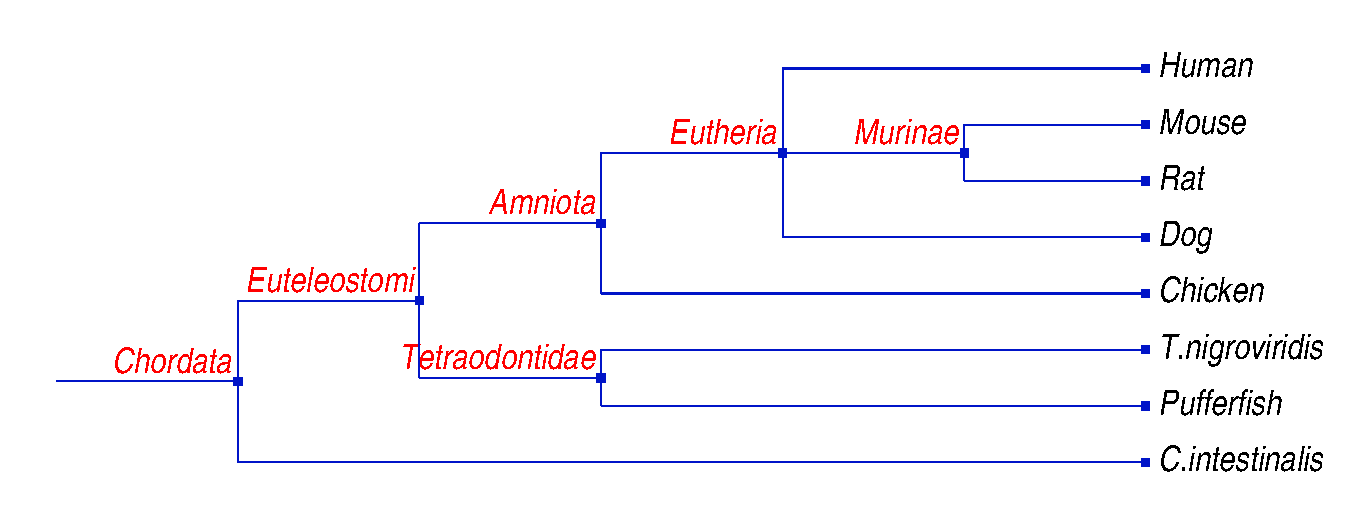
\includegraphics[width=\textwidth]{spec}}
	{\hyperlink{gene-tree}{\beamergotobutton{gene tree}}}
}
\frame {
	\frametitle{Gene families and orthologs}
	\begin{itemize}
		\item \alert{Gene family} is a group of gene that are descendant from a single gene.
		\item \alert{Homologs} are genes that are descendant from a signle gene.
		\item \alert{Orthologs} are genes in different species that originate from a single
			gene in the last common ancestor of these species.
		\item Homologs that are not orthologs are \alert{paralogs}.
	\end{itemize}
}
\frame {
	\frametitle{Interpretting the history of gene evolution}
	{\center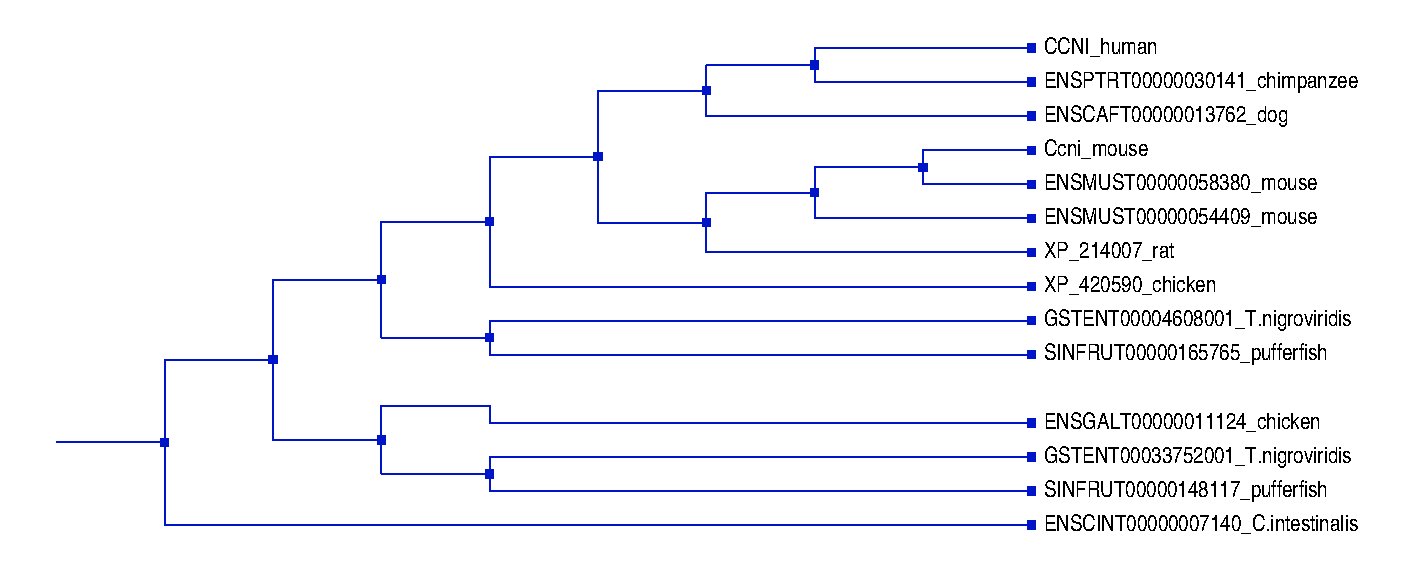
\includegraphics[width=\textwidth]{gtree-plain}}
	\begin{itemize}
	\item {\sf CCNI\_human} and {\sf XP\_420590\_chicken} are orthologs.
	\item {\sf CCNI\_human} and {\sf ENSGALT00000011124\_chicken} are paralogs.
		({\it See also} \hyperlink{spec-tree}{\beamergotobutton{species tree}})
	\end{itemize}
}
\frame {
	\frametitle{Interpretting the history of gene evolution}
	\hypertarget{gene-tree}{}
	{\center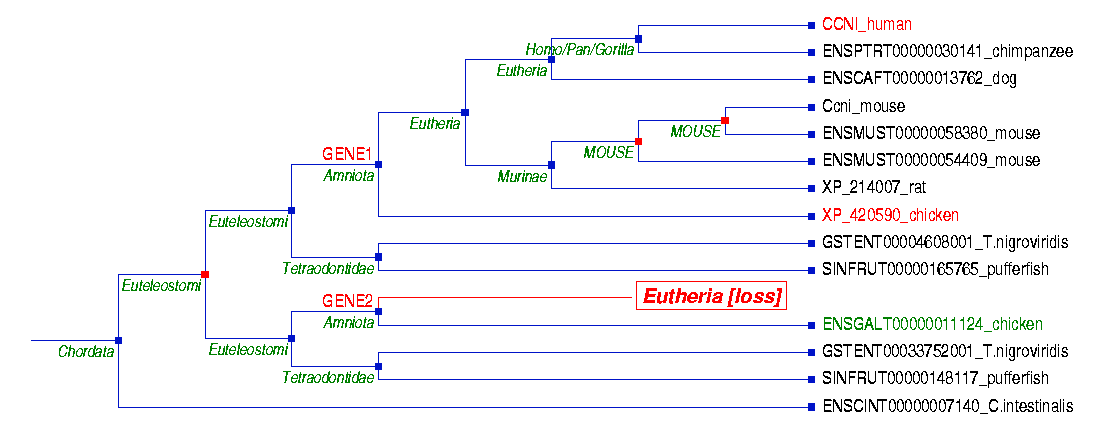
\includegraphics[width=\textwidth]{gtree}}
	\begin{itemize}
	\item {\sf CCNI\_human} and {\sf XP\_420590\_chicken} are orthologs.
	\item {\sf CCNI\_human} and {\sf ENSGALT00000011124\_chicken} are paralogs.
		({\it See also} \hyperlink{spec-tree}{\beamergotobutton{species tree}})
	\end{itemize}
}
\frame {
	\frametitle{Why is gene evolution important?}
	\begin{itemize}
	\item Transfer gene annotations across different species.
	\item Gene evolution is subjected to functional shifts and, in turn, reflects functional implication.
		\begin{itemize}
		\item Infer meaningful mutations.
		\item Detect pseudogenes and genes under positive selections.
		\item Reconstruct protein-protein interaction networks.
		\end{itemize}
	\item Pave the way for other related evolutionary studies.
		\begin{itemize}
		\item Intron evolution
		\item Genome-wide duplications
		\end{itemize}
	\end{itemize}
}
\subsection{What is TreeFam?}
\frame {
	\frametitle{What is TreeFam?}
	\begin{itemize}
	\item \alert{TreeFam} is a database of curated phylogenetic trees of animal gene families.
		\begin{itemize}
		\item A protein classification database: classify genes into families,
			and assign a name to each family and significant subfamilies.
		\item An ortholog database: infer orthologs and paralogs from the phylogenetic tree
			of a gene family.
		\item A curated database: contain manually curate phylogenetic trees.
		\end{itemize}
	\end{itemize}
}
\frame {
	\frametitle{Protein classification}
	\begin{itemize}
	\item Existing databases: KOG, PANTHER, SYSTERS and PhIGs
	\item Conventional strategy: except PhIGs, most of them define families according to
		the degree of similarities between family members.
	\item Disadvantages of conventional methods:
		\begin{itemize}
		\item sensitive to the threshold that is used at clustering stage.
		\item lack biological meaning
		\end{itemize}
	\item TreeFam strategy: an (animal) gene family is a group of genes that descended from a single gene
		in the last common ancestor of all metazoan animal, or that first appeared in metazoan animals.
	\end{itemize}
}
\frame {
	\frametitle{Ortholog assignment}
	\begin{itemize}
	\item Existing databases: NCBI HomoloGene, Ensembl-Compara, OrthoMCL, Inparanoid and HOGENOM
	\item Conventional strategy: except HOGENOM, most of them infer orthologs from pairwise alignment between
		two species.
	\item Disadvantages of conventional methods:
		\begin{itemize}
		\item Inconsistent across several species: for example, if gene $g_1$ and $g_2$ are
			1:1 orthologs and $g_2$ and $g_3$ are also 1:1 orthologs, conventional
			method may still infer that $g_1$ and $g_3$ are paralogs.
		\item Lead to incorrect results when losses occur.
		\item Hard to manually check whether ortholog assignments are correct.
		\end{itemize}
	\item TreeFam strategy: infer orthologs from phylogenetic trees.
	\end{itemize}
}
\frame {
	\frametitle{Curated resources}
	\begin{itemize}
	\item All existing databases are automatically generated.
	\item Correctly reconstructing phylogenetic trees is very difficult.
	\item TreeFam strategy: visualize phylogenies as a tree and let experts
		curate the topology of the tree. Do all inferences from phylogenetic trees.
	\end{itemize}
}
\subsection{Difficulties in Constructing the TreeFam}
\frame {
	\frametitle{Four algorithms inspired by TreeFam}
	\begin{itemize}
	\item Reserving manual curation\uncover<2>{: constrained neighbour-joining}
	\item Better automatic trees\uncover<2>{: tree merge algorithm}
	\item Ortholog inference for multifurcated species trees\uncover<2>{: DLI for multifurcated species trees}
	\item Visualization of trees\uncover<2>{: leaf reordering algorithm}
	\end{itemize}
}
\frame {
	\frametitle{Difficulties: curation}
	\begin{alertblock}{Problem}
		Curation on topologies must be reserved when reconstructing trees, \alert{but} all
		the existing methods are unsupervised.
	\end{alertblock}
	\begin{block}{Solution}
		\alert{Constrained neighbour-joining} algorithm that adds new sequences to
		an existing tree without changing the given topology.
	\end{block}
}
\frame {
	\frametitle{Difficulties: reconstructing reliable trees}
	\begin{alertblock}{Problem}
		\begin{itemize}
		\item Sequences of poor qualities: incorrect gene annotations or few informative sites.
		\item Unrealistic evolutionary model: assuming different lineages evolved at the same rate.
		\end{itemize}
	\end{alertblock}
	\begin{block}{Solutions}
		\begin{itemize}
		\item Sophisticated single-model algorithms such as maximum likelihood (ML) and maximum parsimony (MP) methods.
		\item \alert{Tree merge algorithm}.
		\item Manual curation.
		\end{itemize}
	\end{block}
}
\frame {
	\frametitle{Difficulties: inference given a multifurcated species tree}
	\begin{alertblock}{Problem}
		Most of algorithms that infer orthologs only work with a binary species tree, \alert{but}
		the most widely used NCBI species tree is multifurcated.
	\end{alertblock}
	\begin{block}{Solution}
		\alert{Duplication/loss inference (DLI)} for a multifurcated species tree.
	\end{block}
}
\frame {
	\frametitle{Difficulties: visualization of trees}
	\begin{alertblock}{Problem}
		The same tree can be drawed in different ways depending on
		the order of its leaves, \alert{but} they may look quite different in human's eyes.
	\end{alertblock}
	\begin{block}{Solution}
		\alert{Leaf reordering algorithm} that plots a tree in a determined way.
	\end{block}
}

%
%
%

\section{Constructing the TreeFam Database}
\subsection{Contents and basic structures}
\frame {
	\frametitle{Philosophy}
	\begin{itemize}
	\item Two parted databases:
		\begin{itemize}
		\item TreeFam-A: curated
		\item TreeFam-B: automatically generated
		\end{itemize}
	\item Two types sequences and trees:
		\begin{itemize}
		\item seed: either from curation (for TreeFam-A) or from PhIGs clusters (for TreeFam-B).
		\item full: also including new sequences that are added to the corresponding seed.
		\end{itemize}
	\end{itemize}
}
\frame {
	\frametitle{Status of TreeFam-2}
	\begin{itemize}
		\item 1174 TreeFam-A families (curated)
		\item 15254 TreeFam-B families (automatic)
		\item 19 species, including 16 metazoan animals
		\item 93\% coverage of all mammalian coding genes
	\end{itemize}
}
\subsection{Automatic Pipelines}
\frame {
	\frametitle{Flowchart}
	\begin{center}
	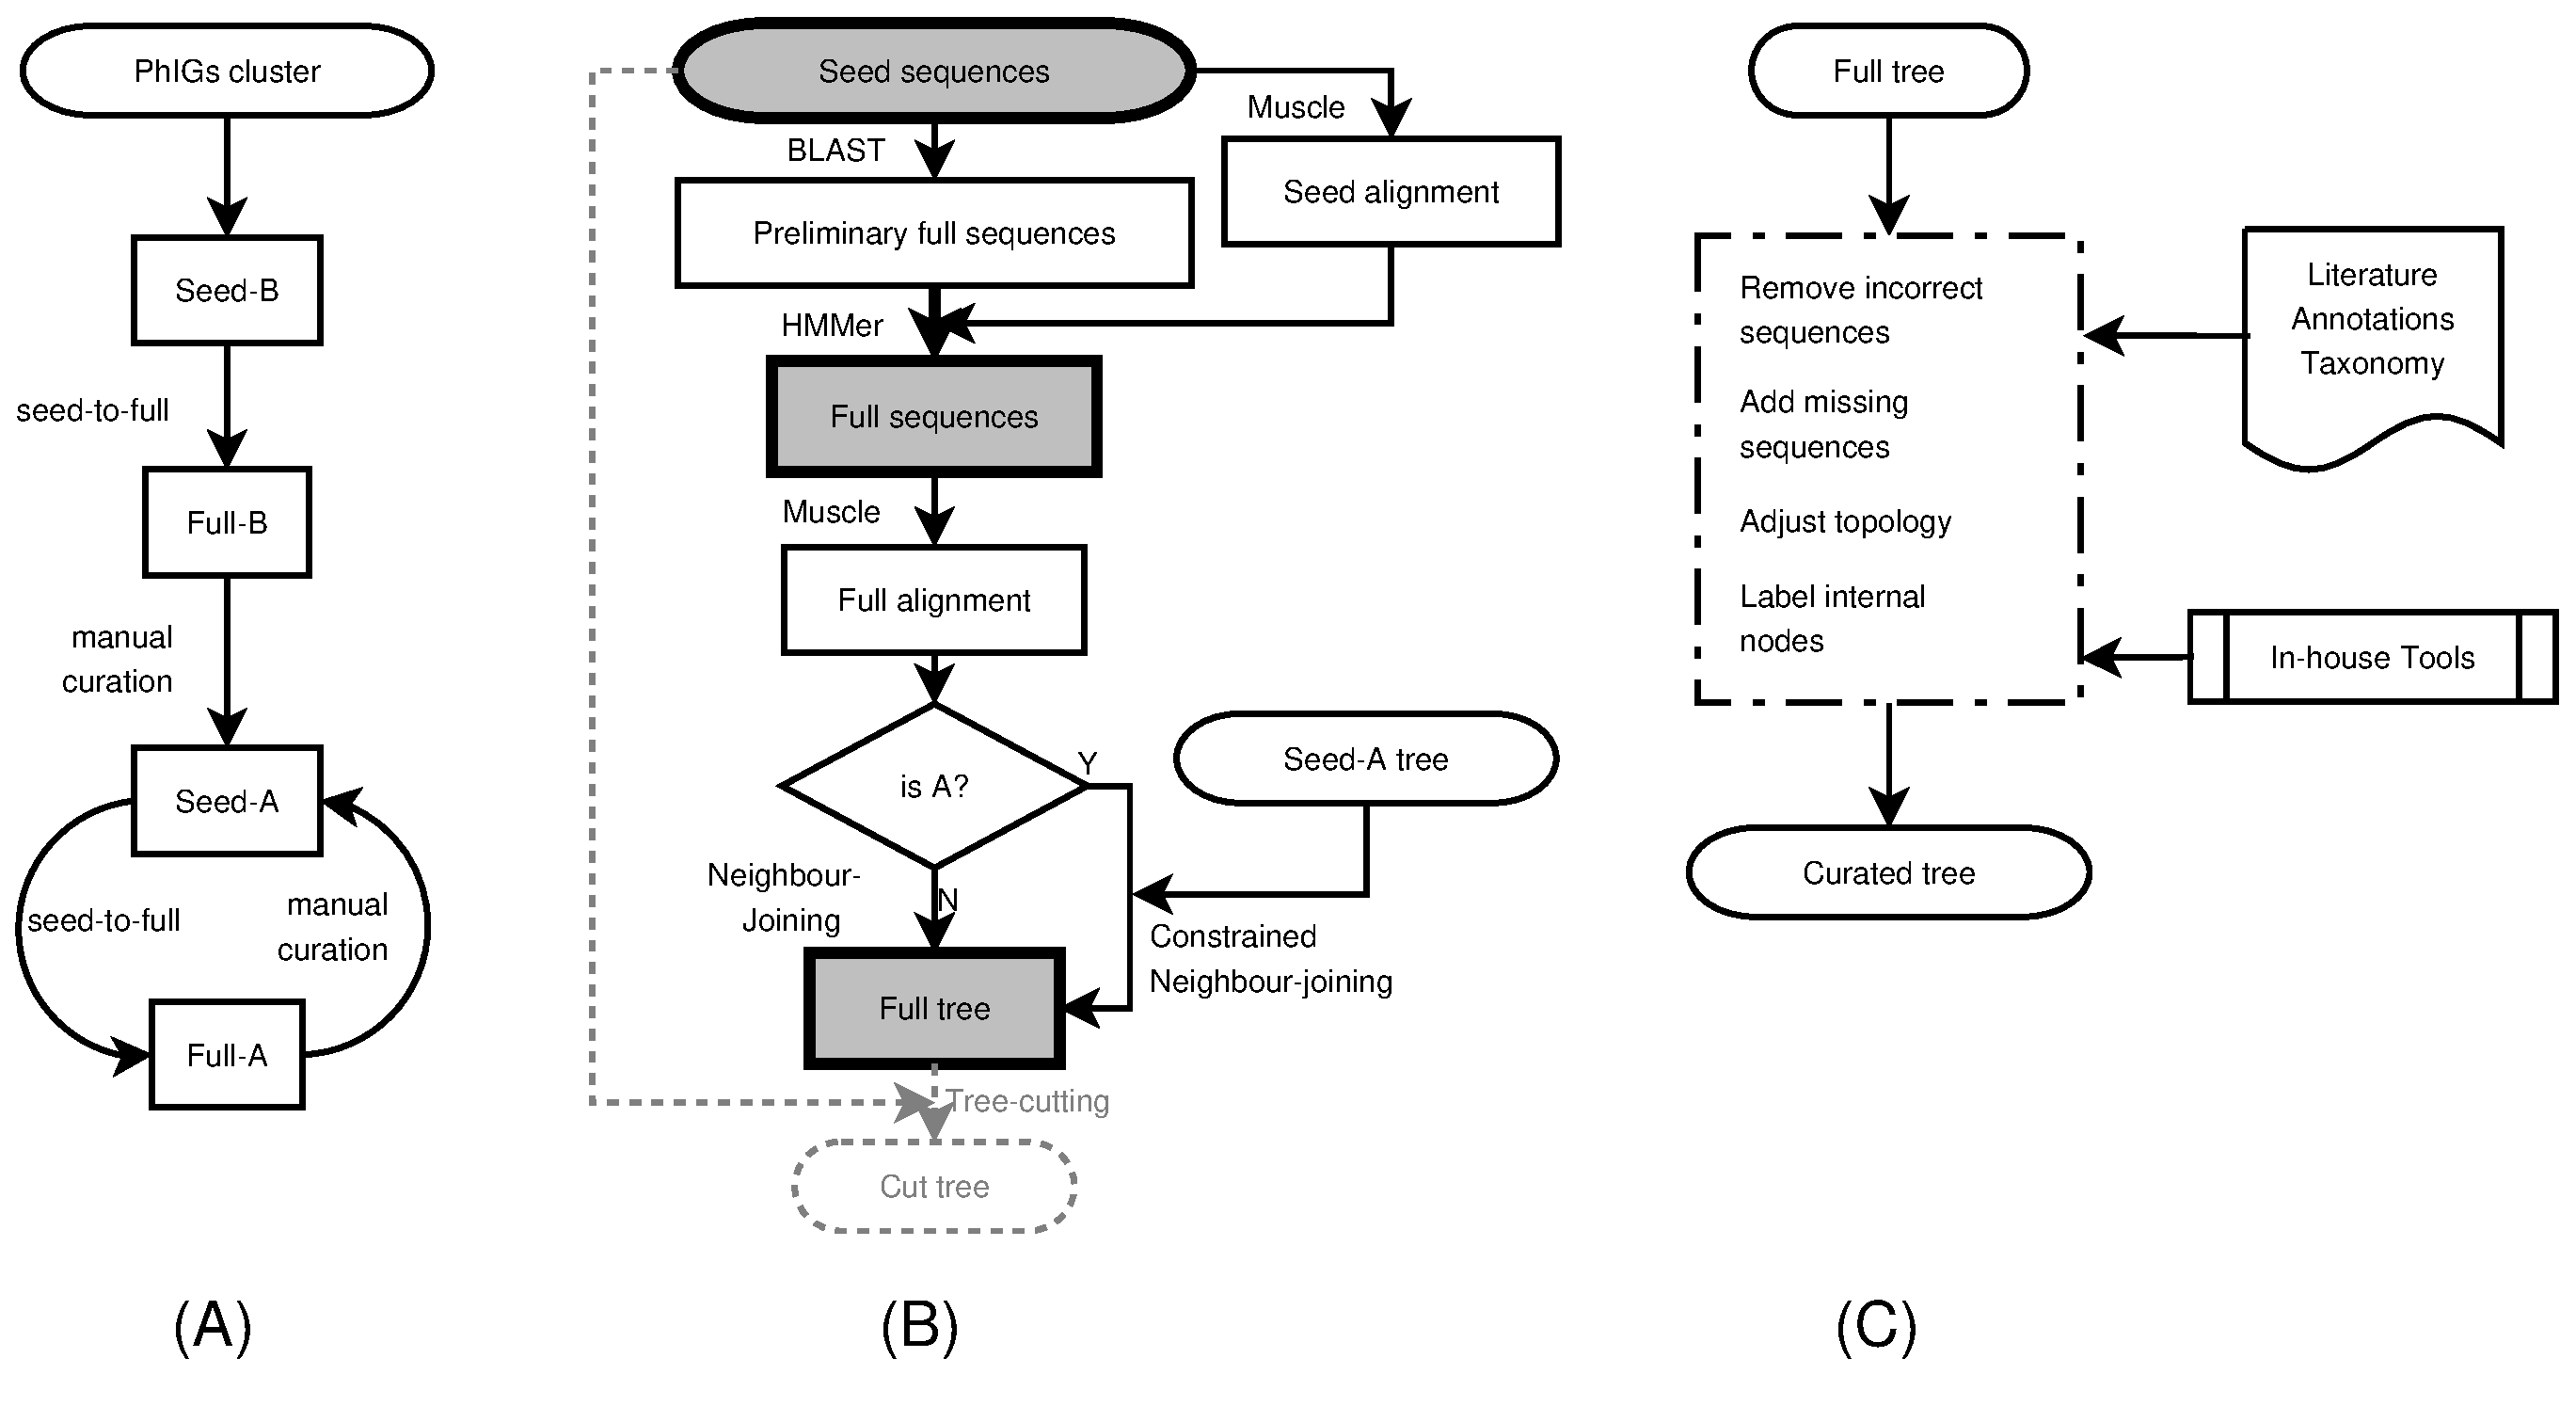
\includegraphics[width=\textwidth]{flowchart}
	\end{center}
}
\frame {
    \frametitle{Constructing TreeFam-B seeds}
    \begin{itemize} 
        \item Given PhIGs cluster $u$, let $R_u\in u$ be the set of animal genes whose
            HMMER bit-scores are higher than scores of any outgroup genes in $u$.
        \item An edge $[u,v]$ is added if $R_u\cap R_v\not=\emptyset$.
        \item Weight $w_{uv}=\frac{|R_u\cap R_v|}{\min\{|R_u|,|R_v|\}}$.
        \item Find groups in which edges tend to be saturated.
        \item Only one round is applied.
		\item The final groups are used as seeds.
    \end{itemize}
}
\frame {
	\frametitle{Seed-to-full expansion}
	\begin{itemize}
	\item BLAST seed sequences against the whole TreeFam sequence set (TFSEQ).
	\item Refine matched sequences with HMMER. HMM profiles are built from seed multialignment by MUSCLE.
	\item One {\it sequence} (or one transcript) is arbitrarily assigned to one family.
		One {\it gene} can be present in several.
	\end{itemize}
}
\frame {
	\frametitle{Reconstructing trees}
	\begin{itemize}
	\item Automatic full trees for TreeFam-B families
	\item Automatic `clean' trees for all families (tree merge)
	\item TreeFam-A full trees reconstructed by constrained neighbour-joining
	\item Branch lengths are estimated by ML algorithm combined with HKY model
	\end{itemize}
}


\section{TreeFam Related Algorithms}
\subsection{Constrained Neighbour-Joining}
\frame {
	\frametitle{Neighbour-joining algorithm}
	\begin{itemize}
	\item Neighbour-joining (NJ) reconstructs a tree from a distance matrix $(d_{ij})_{n\times n}$
	\item NJ joins a neighbour pair at each step.
	\item A \alert{neighbour} is the leaf pair that minimizes $D_{ij}$:
		\[D_{ij}=d_{ij}-(r_i+r_j)\]
		\[r_i = \frac{1}{n-2}\sum_{k=1}^n d_{ik}\]
	\item The dimension of $(d_{ij})$ is reduced by 1 at each step.
	\item Constrained neighbour-joining (cNJ) only joins a pair of leaves that are constrained or share
		the same adjacent node of the constraining tree.
	\end{itemize}
}
\frame {
	\frametitle{Standard neighbour-joining}
	\begin{overprint}
		\onslide<1>\begin{center}\includegraphics{mpfig.11}\end{center}
		\onslide<2>\begin{center}\includegraphics{mpfig.12}\end{center}
		\onslide<3>\begin{center}\includegraphics{mpfig.13}\end{center}
		\onslide<4>\begin{center}\includegraphics{mpfig.1}\end{center}
	\end{overprint}
	\begin{itemize}
	\item<2-> {\color{red} Step 1}: add 6 that joins 1 and 2
	\item<3-> {\color{darkgreen} Step 2}: add 7 that joins 3 and 4
	\item<4> {\color{darkblue} Step 3}: add 8 that joins the rest
	\end{itemize}
}
\frame {
	\frametitle{Constrained neighbour-joining}
	\begin{overprint}
		\onslide<1>
		\begin{center}
		\includegraphics{mpfig.3}
		\hspace{1cm}
		\includegraphics{mpfig.12}
		\end{center}
		\onslide<2>
		\begin{center}
		\includegraphics{mpfig.3}
		\hspace{1cm}
		\includegraphics{mpfig.13}
		\end{center}
		\onslide<3>
		\begin{center}
		\includegraphics{mpfig.3}
		\hspace{1cm}
		\includegraphics{mpfig.15}
		\end{center}
		\onslide<4>
		\begin{center}
		\includegraphics{mpfig.3}
		\hspace{1cm}
		\includegraphics{mpfig.2}
		\end{center}
	\end{overprint}
	\begin{itemize}
	\item<1-> {\color{red} Step 1}: add 6 that joins 1 and 2 (no constraint)
	\item<3-> {\color{darkgreen} Step 2}: add 9 that joins 4 and 5 (\alert<3>{joining 3 and 4 is disallowed})
	\item<4-> {\color{darkblue} Step 3}: add 10 that joins the rest
	\end{itemize}
}
\subsection{Leaf Reordering Algorithm}
\frame {
	\begin{center}
	\begin{overprint}
	\onslide<1>
	\includegraphics[width=10cm]{mpfig.5}
	\onslide<2>
	\includegraphics[width=10cm]{mpfig.6}
	\end{overprint}
	\end{center}
}
\frame {
	\frametitle{Leaf Reordering}
	\begin{itemize}
	\item Goal: Plot similar trees in similar manners.
	\item Philosophy: find a way of plotting to minimize a certain objective function.
	\item Objective function: draw a tree in the way that minimizes $\sum_i{(i-w_i)^2}$ where
		$w_i$ is the weight of $i$-th leaf shown in the image of the tree.
	\item Algorithm: switch the left subtree and the right one at the node where
		the average weight in the left subtree is larger than the weight in the right subtree.
	\item Time complexity: $O(N)$
	\end{itemize}
}
\subsection{Duplication/Loss Inference}
\frame {
	\frametitle{Example of duplications and losses}
	\begin{center}
	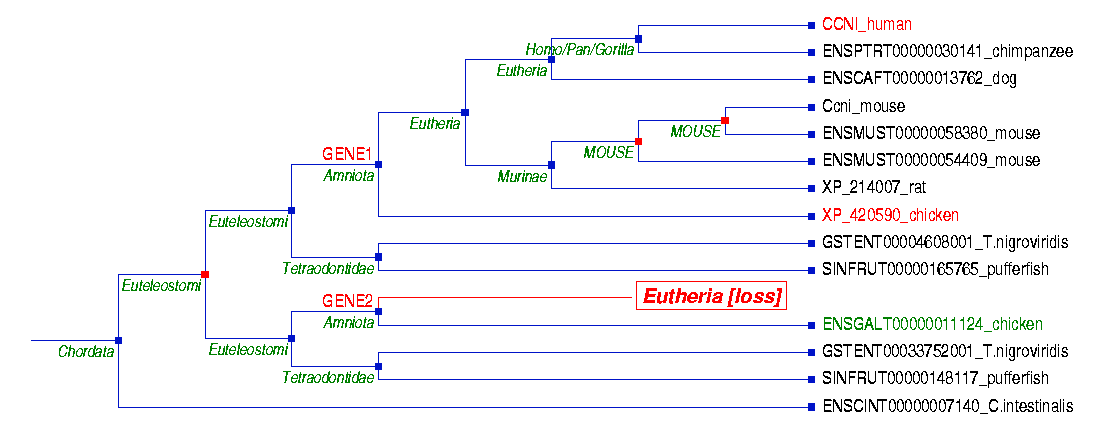
\includegraphics[width=\textwidth]{gtree}
	\end{center}
	\hyperlink{spec-tree}{\beamergotobutton{species tree}}
}
\frame {
	\frametitle{Inferring duplications and losses}
	\begin{itemize}
	\item $\bar{g}=\{g':\mbox{leaf $g'$ is a descendant of $g$}\}$
	\item Parsimonious duplication function $D^*(\bar{g}_1,\bar{g}_2)$: $D^*$ equals to 1
		if the node represented by $\bar{g}_1\cup\bar{g}_2$ is a duplication; otherwise euqals to 0.
	\item Parsimonious loss function $L^*(\bar{g}_1,\bar{g}_2)$: the number of minimum losses
		when the node represented by $\bar{g}_1\cup\bar{g}_2$ evolved into its two daughters
		that are represented by $\bar{g}_1$ and $\bar{g}_2$, respectively.
	\end{itemize}
}
\frame {
	\frametitle{Example of DLI}
	\begin{overprint}
	\onslide<1>
	\begin{center}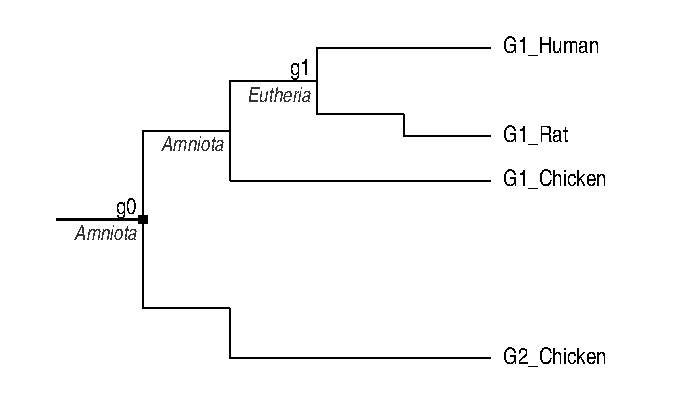
\includegraphics[width=0.5\textwidth]{dli-exa-plain}\end{center}
	\onslide<2>
	\begin{center}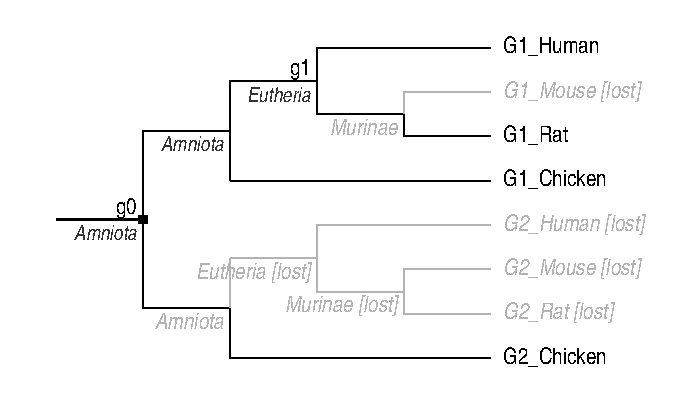
\includegraphics[width=0.5\textwidth]{dli-exa}\end{center}
	\end{overprint}
	\begin{overprint}
	\onslide<2-3>
	\begin{itemize}
	\item $D^*(\{\mbox{G2\_Chicken}\},\{\mbox{G1\_Human,G1\_Rat,G1\_Chicken}\})=1$
	\item $L^*(\{\mbox{G2\_Chicken}\},\{\mbox{G1\_Human,G1\_Rat,G1\_Chicken}\})=1$
	\item $D^*(\{\mbox{G1\_Human}\},\{\mbox{G1\_Rat}\})=0$
	\item $L^*(\{\mbox{G1\_Human}\},\{\mbox{G1\_Rat}\})=1$
	\end{itemize}
	\end{overprint}
}
\subsection{Tree Merge Algorithm}
\frame {
	\frametitle{Set representation}
	\begin{center}\includegraphics{mpfig.10}\end{center}
	\begin{itemize}
	\item $V=\{1,2,3,4,5\}$
	\item $\bar{g}=\{1,2,3\}$
	\item $\bar{G}=\{\{1\},\{2\},\{3\},\{4\},\{5\},\{2,3\},\{1,2,3\},\{1,2,3,4\},V\}$
	\end{itemize}
}
\frame {
	\frametitle{Tree merge problem}
	\begin{block}{Problem}
		Given a set of binary rooted trees with the same leaf set $V$, reconstruct
				a binary rooted tree such that:
			\begin{itemize}
			\item each branch of the resultant tree comes from one of the given trees
			\item the resultant tree minimizes a \alert<2->{certain} objective function
			\end{itemize}
	\end{block}
	\begin{overprint}
	\onslide<2>
	Required properties of the objective function:
	\begin{itemize}
	\item additivity
	\item topological independence
	\end{itemize}
	\[F(\bar{G})=\sum_{\bar{g}\in \bar{G}}f({\rm chi}(\bar{g}))=\sum_{\bar{g}\in \bar{G}}f(\bar{g}_1,\bar{g}_2)\]
	\onslide<3>
	Things can be considered in the objective function:
	\begin{itemize}
	\item higher bootstrapping supports at each branch ($B^*$)
	\item smaller number of duplications and losses inferred by using parsimonious species map ($D^*$ and $L^*$)
	\item the advantage of different algorithms (indirectly, via $B^*$)
	\end{itemize}
	\[f(\bar{g}_1,\bar{g}_2)=f(\bar{g}_2,\bar{g}_1)=\alpha D^*(\bar{g}_1,\bar{g}_2)
	    +\beta L^*(\bar{g}_1,\bar{g}_2)-\gamma B^*(\bar{g}_1,\bar{g}_2)\]
	\end{overprint}
}
\frame {
	\frametitle{Tree merge algorithm}
	\begin{overprint}
	\onslide<1>
	\begin{itemize}
	\item Construct the set of all branches:
		\[\Phi=\{\bar{G}_1,\bar{G}_2,\ldots,\bar{G}_n\}\]
		\[\mathcal{G}(\Phi)=\bigcup_{\bar{G}'\in\Phi} \bar{G'}\]
	\item Convert the optimization process to the calculation of a function $F^*(V)$:
		\[F^*(\bar{g}) = \min_{\bar{G}|_{\bar{g}}\in\Omega(\mathcal{G}|_{\bar{g}})} F(\bar{G}|_{g})\]
		\[F^*(V) = \min_{\bar{G}\in\Omega(\mathcal{G})} F(\bar{G})\]
	\end{itemize}
	\onslide<2>
	\begin{itemize}
	\item Construct permitted children pairs given a node $\bar{g}$:
		\[\mathcal{C}(\bar{g}) = \left\{\{\bar{g}_1,\bar{g}_2\}:\mbox{$\bar{g}_1,\bar{g}_2\in
			\mathcal{G}$, $\bar{g}_1\cap\bar{g}_2=\emptyset$ and $\bar{g}_1\cup\bar{g}_2=\bar{g}$}\right\}\]
	\item Recursively calculate all $F^*(\bar{g})$:
		\[F^*(\bar{g}) = \min_{\{\bar{g}_1,\bar{g}_2\}\in\mathcal{C}(\bar{g})}\left\{F^*(\bar{g}_1)+
			f(\bar{g}_1,\bar{g}_2)+F^*(\bar{g}_2)\right\}\]
	\end{itemize}
	\end{overprint}
}
\frame {
	\begin{center}
	\includegraphics[width=0.9\textwidth]{mpfig.7}
	\end{center}
}
\frame {

{\footnotesize\center
	\begin{tabular}{|l|l|}
	\hline
	Type & Comments \\
	\hline
	{\tt CUR} & Curated trees from TreeFam \\
	\hline
	{\tt NJ-NT-HKY4} & Neighbour-Joining, HKY model, $C=4$, $\alpha=1.0$, $\kappa$ estimated \\
	{\tt NJ-AA-WAG4} & Neighbour-Joining, WAG model, $C=4$, $\alpha=1.0$ \\
	{\tt NJ-NT-dN} & NJ, non-synonymous distance, no correction for multi-substitutions \\
	{\tt NJ-NT-dS} & NJ, synonymous distance, no correction for multi-substitutions \\
	{\tt NJ-AA-MM} & NJ, p-distance (or mismatch) distance, no correction \\
	{\tt NJ-AA-Kmr} & NJ, with Kimura correction \\
	{\tt ME-NT-HKY4} & FastME, HKY model, $C=4$, $\alpha=1.0$, $\kappa$ estimated \\
	{\tt ME-AA-WAG4} & FastME, WAG model, $C=4$, $\alpha=1.0$ \\
	\hline
	{\tt PAR-NT} & Parsimony (dnapars) \\
	{\tt PAR-AA} & Parsimony (protpars) \\
	\hline
	{\tt ML-NT-HKY4} & PHYML, HKY, $C=4$, $\alpha=1.0$, $\kappa$ estimated \\
	{\tt ML-NT-HKY2} & PHYML, HKY, $C=2$, $\alpha=1.0$, $\kappa$ estimated \\
	{\tt ML-NT-HKY1} & PHYML, HKY, $C=1$, $\alpha=1.0$, $\kappa$ estimated \\
	{\tt ML-AA-WAG4} & PHYML, WAG, $C=4$, $\alpha=1.0$ \\
	\hline
	{\tt NJ-NT-dM} & Tree merge from {\tt NJ-NT-dS} and {\tt NJ-NT-dN} \\
	{\tt MERGE} & From {\tt ML-NT-HKY4}, {\tt ML-AA-WAG4}, {\tt NJ-NT-dN} and {\tt NJ-NT-dS}\\
	\hline
	\end{tabular}
}
}

\frame {

{\footnotesize\center
	\begin{tabular}{|l|cc|cc|cc|ccc|}
	\hline
	Type             &$d_M$ &$\sigma$&$p_D$ &$\sigma$&$p_L$ &$\sigma$ \\
	\hline
	{\tt CUR}        & 0.000 & 0.000 & 0.249 & 0.017 & 0.388 & 0.029 \\
	\hline                                                                                   
	{\tt NJ-NT-HKY4} & 0.225 & 0.017 & 0.313 & 0.017 & 0.786 & 0.042 \\
	{\tt NJ-AA-WAG4} & 0.256 & 0.016 & 0.322 & 0.016 & 0.901 & 0.050 \\
	{\tt NJ-NT-dN}   & 0.201 & 0.011 & 0.308 & 0.015 & 0.796 & 0.040 \\
	{\tt NJ-NT-dS}   & 0.527 & 0.017 & 0.431 & 0.014 & 1.761 & 0.041 \\
	{\tt NJ-AA-MM}   & 0.225 & 0.012 & 0.308 & 0.016 & 0.823 & 0.042 \\
	{\tt NJ-AA-Kmr}  & 0.275 & 0.018 & 0.333 & 0.017 & 0.988 & 0.065 \\
	{\tt ME-NT-HKY4} & 0.200 & 0.015 & 0.307 & 0.017 & 0.720 & 0.035 \\
	{\tt ME-AA-WAG4} & 0.232 & 0.014 & 0.317 & 0.017 & 0.858 & 0.047 \\
	\hline
	{\tt PARS-NT}    & 0.203 & 0.013 & -     & -     & -     & -     \\
	{\tt PARS-AA}    & 0.181 & 0.013 & 0.286 & 0.016 & 0.614 & 0.035 \\
	\hline
	{\tt ML-NT-HKY4} & 0.152 & 0.017 & 0.300 & 0.016 & 0.676 & 0.041 \\
	{\tt ML-NT-HKY2} & 0.147 & 0.018 & 0.301 & 0.017 & 0.677 & 0.041 \\
	{\tt ML-NT-HKY1} & 0.172 & 0.017 & 0.306 & 0.016 & 0.693 & 0.038 \\
	{\tt ML-AA-WAG4} & 0.185 & 0.015 & 0.299 & 0.016 & 0.705 & 0.044 \\
	\hline
	{\tt NJ-NT-dM}   & 0.165 & 0.011 & 0.291 & 0.016 & 0.687 & 0.037 \\
	{\tt MERGE}      & 0.092 & 0.015 & 0.259 & 0.016 & 0.457 & 0.033 \\
	\hline
	\end{tabular}
}
}



\section*{Acknowledgement}
\frame {
	\frametitle{Acknowledgement}
	\begin{itemize}
	\item Zheng Wei-mou (supervisor)
	\item Wang Jun (header of bioinformatics division of BGI)
	\item Richard Durbin (header of informatics division of Sanger)
	\item Liu Tao
	\item Avril Coghlan, Jean-Karim H\'{e}rich\'{e}, Lachlan James Coin, and Alan Moses (developers of Sanger)
	\item Hao Bai-lin and Guo Ling
	\item all my friends in BGI and ITP
	\item my parents and my wife
	\end{itemize}
}
\frame {
	\begin{center}
	{\Huge Thank You!}
	\end{center}
}

\end{document}
